\documentclass[11pt]{article}
\title{\LARGE{\bf \textsf{CS550: Massive Data Mining and Learning}}\\ {\bf \textsf{Homework 2}}}
\author{Christos Mitropoulos - cm1012 \\ email \href{mailto:c.mitro@rutgers.edu}{c.mitro@rutgers.edu} \\\\ Github repository:\\ \href{https://github.com/CMitropoulos/MassiveDataMining/tree/master/Homework3}{https://github.com/CMitropoulos/MassiveDataMining/tree/master/Homework3}}
\date{}
\usepackage{fullpage}
\usepackage{url}
\usepackage{listings}
\usepackage{amsmath}
\usepackage{hyperref}
\usepackage{comment}
\usepackage{graphicx}
\usepackage{float}

\begin{document}
\begin{titlepage}
\maketitle
\end{titlepage}

\pagebreak[4]
\begin{center}
\LARGE{\bf \textsf{Submission Instructions}} \\*[4ex]
\end{center}

\textbf{Assignment Submission } Include a signed agreement to the Honor Code with this assignment. Assignments are due at 11:59pm. All students must submit their homework via Sakai. Students can typeset or scan their homework. Students also need to include their code in the final submission zip file. Put all the code for a single question into a single file. 
\\
\\
\textbf{Late Day Policy } Each student will have a total of {\em two} free late days, and for each homework only one late day can be used. If a late day is used, the due date is 11:59pm on the next day.
\\
\\
\textbf{Honor Code } Students may discuss and work on homework problems in groups. This is encouraged. However, each student must write down their solutions independently to show they understand the solution well enough in order to reconstruct it by themselves.  Students should clearly mention the names of all the other students who were part of their discussion group. Using code or solutions obtained from the web is considered an honor code violation. We check all the submissions for plagiarism. We take the honor code seriously and expect students to do the same. 

\vfill
\vfill

Discussion Group (People with whom you discussed ideas used in your answers): \\\\\\
On-line or hardcopy documents used as part of your answers: \\\\\\
\vfill

\vfill

I acknowledge and accept the Honor Code.\\*[3ex]
\bigskip
\textit{(Signed)}
Christos Mitropoulos 
\vfill
\vfill

\pagebreak[4]
\section*{Answer to Question 1,2}
The graphs and the plots were created with networkx python library. The code will be also attached as graphs.py.
\section*{Answer to Question 1(a)}
\begin{figure}[h]
\caption{This is the Graph after removing the edge (A, G).}
\centering
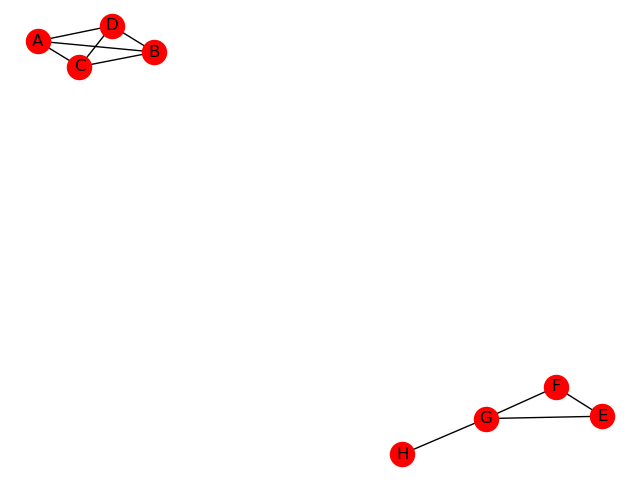
\includegraphics[width=0.5\textwidth]{./figures/G_a}
\end{figure}
Modularity =  -0.14049586776859507

\section*{Answer to Question 1(b)}
\begin{figure}[h]
\caption{This is the Graph after adding the edge (E, H).}
\centering
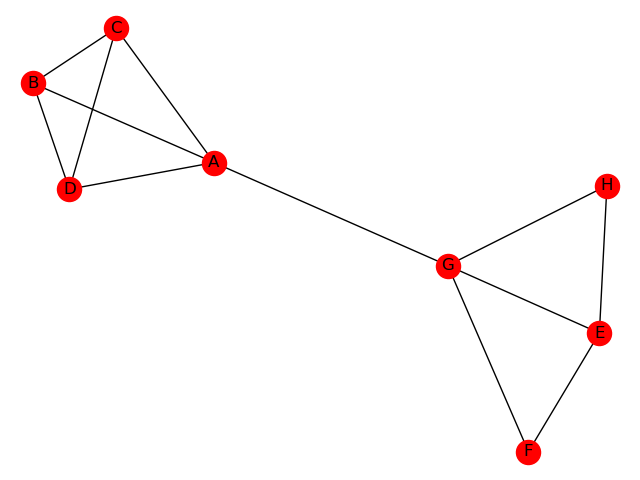
\includegraphics[width=0.5\textwidth]{./figures/G_b}
\end{figure}
Modularity =  -0.13194444444444442

We see that the modularity was increased. This can be explained by the extra edge added in one of the groups identified before. This makes the group stronger and therefore the overall modularity is increased.

\section*{Answer to Question 1(c)}
\begin{figure}[h]
\caption{This is the Graph after adding the edge (F, A).}
\centering
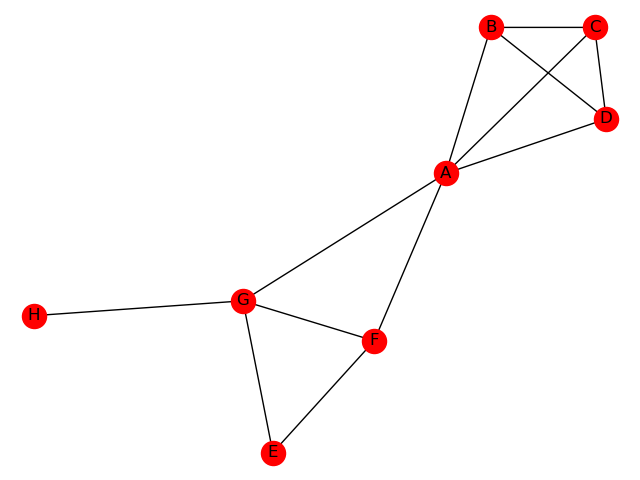
\includegraphics[width=0.5\textwidth]{./figures/G_c}
\end{figure}
Modularity =  -0.14236111111111108

We see that the modularity decreased. This can be explained by the edge that we added. This edge connects two nodes that belong to different groups and therefore the groups become less strong and therefore the modularity decreases.


\section*{Answer to Question 2(a)}
Adjacency matrix: 
\begin{figure}[h]
\centering
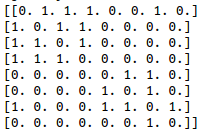
\includegraphics[width=0.5\textwidth]{./figures/adjacency}
\end{figure}

Degree matrix:\\
{'A': 4, 'B': 3, 'C': 3, 'D': 3, 'E': 2, 'F': 2, 'G': 4, 'H': 1}\\

Laplacian matrix: 
\begin{figure}[h]
\centering
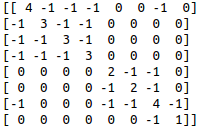
\includegraphics[width=0.5\textwidth]{./figures/Laplacian}
\end{figure}

\section*{Answer to Question 2(b)}
Laplacian eigenvalues:
\begin{figure}[h]
\centering
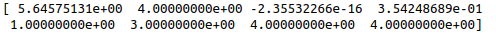
\includegraphics[width=0.8\textwidth]{./figures/L_eigval}
\end{figure}

Laplacian eigenvectors:
\begin{figure}[h]
\centering
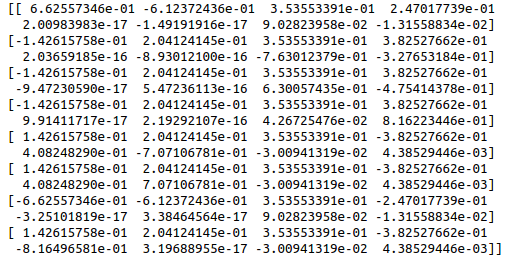
\includegraphics[width=0.8\textwidth]{./figures/L_eigvec}
\end{figure}

\section*{Answer to Question 2(c)}
This is the eigenvector for the second smallest eigenvalue:\\
$[0.24701774,  0.38252766,  0.38252766,  0.38252766, -0.38252766, -0.38252766, -0.24701774, -0.38252766]$ \\
Using 0 as boundary we partition the graph into two communities. The first community contains the nodes that have negative eigenvector value and the second community contains the nodes that have a positive eigenvector value. \\
Thus the graph partitioning is the following: \\
Nodes A, B, C, D belong to the first community and nodes E, F, G, H belong to the second community.
\section*{Answer to Question 3(a)}
By definition $C_i$ is a clique if there are fewer than two nodes in it. 
In any other case, any two nodes in $C_i$ have an edge between them since they have i as a common factor.
\section*{Answer to Question 3(b)}
i must be a prime number $\leq$ 1,000,000 
\begin{itemize}
\item If i is $\leq$ 1,000,000 but isn't prime, let j be a factor of i and 
1 < j < i. Node j is not in $C_i$, however it has an edge to every member of $C_i$, since it has j as a common factor. Therefore, $C_i$ is not maximal.
\item If i is $\geq$ 1,000,000  then $C_i$ is the empty clique and adding one node will make it a 1-clique, which is not maximal.
\item If i is prime and $\leq$ 1,000,000 then there is no node outside $C_i$ that has an edge to the node i itself. Suppose there was a node j like that. Then i and j have a common factor other than 1, which can only be i, since i is prime. This makes j a multiple of i since j has i as a factor and therefore j is already in $C_i$.
\end{itemize}
\section*{Answer to Question 3(c)}
i and i+1 are always relatively prime. If they had a common factor p>1 then (i+1) - i =1 must also be divisible by p and this is impossible for any p>1.
Only one of the {2,3},{4,5},{6,7},{8,9},... can be in a clique. The largest possible clique has 500,000 members as $C_2$.\\
There are no cliques other than $C_2$ that have 500,000 members. For a clique to have 500,000 members, it must contain 2 or 3, since otherwise the clique will have at most 499,999 members. If it contains 3, then all other members must have 3 as a factor (3 being a prime) and there less than 499,999 elements that are divisible by 3.

\end{document}

